\chapter{Zložitosť}
\label{sect:zlozitost}
\def\longCharts{1}

Keď máme niečo naprogramovať, väčšinou je viac možností, ako to urobiť. A nie všetky sú 
rovnako dobré. Fibonacciho čísla z úlohy~\ref{uloha:Fibonacci} môžem naprogramovať
dvoma spôsobmi takto:


\begin{column}{0.45}
\begin{lstlisting}[] 
long int Fib1(int n) {
  if (n < 3) return n - 1;
  long int a = 0, b = 1, c;
  int i;
  for (i = 2; i < n; i++) {
    c = a + b;
    a = b;
    b = c;
  }
  return c;
}
\end{lstlisting}
\end{column}
\hfil
\begin{column}{0.45}
\begin{lstlisting}[] 
long int Fib2(int n) {
  if (n < 3) return n - 1;
  return Fib2(n - 1) + Fib2(n - 2);
}
\end{lstlisting}
\end{column}


Rekurzívna verzia vpravo je kratšia a lepšie pochopiteľná, lebo z nej priamo vidíme
postup \cmd{$n$-té číslo vyrátaš tak, že sčítaš dve predchádzajúce}.
Má to ale háčik. Začal som si merať čas, koľko trvá, kým sa vyráta $n$-té číslo. 
Funkcia \prg!Fib1! všetky čísla po $90$ (cca toľko sa zmestí do \prg!long int!) vyrátala
pod jednu milisekundu. Pri funkcii \prg!Fib2! som sa dostal po $54$-té číslo. Tam to trvalo
cca 518 sekúnd a potom ma to prestalo baviť. Tu vidíš graf, ako závisel čas behu od veľkosti
$n$. Čísla \vb{Fib2(90)} by som sa nedočkal ani do konca vesmíru.\\


\begin{tikzpicture}
\begin{axis}[
  width=\textwidth, 
  height=10cm,
  xlabel=$n$,
  ylabel=čas (s),
  legend cell align={left},
  legend pos = north west
]
  \addplot+[blue!80!white, 
  line join=round, mark size=0.5pt] table [y=f, x=n]{data/fibcas.dat};
  \addlegendentry{koľko sekúnd trvá vyrátať \vb{Fib2(n)}}
\end{axis}
\end{tikzpicture}


Problém tu bol v tom, že rekurzívna verzia ráta veľa vecí zbytočne: keď chce vyrátať
\vb{Fib2(10)}, najprv ráta \vb{Fib2(9)}. Pri rátaní \vb{Fib2(9)} vyráta 
\vb{Fib2(8)=13}
a \vb{Fib2(7)=8}, takže vráti hodnotu \vb{Fib2(9)=21}. Pokračuje sa v rátaní
\vb{Fib2(10)}: \vb{Fib2(9)} už je vyrátané, ide sa 
 rátať \vb{Fib2(8)}. To sa už síce raz rátalo, ale výsledok
zanikol spolu so svetom predchádzajúceho rekurzívneho volania, takže sa bude rátať
znova. Takto sa nabaľuje veľa 
zbytočnej práce a už aj pre relatívne malé $n$ to začne byť celkom dosť problém.
Napr. na vypočítanie \vb{Fib2(7)} sa v rekurzii postupne vyrobí všetkých $25$ svetov
z nasledujúceho obrázka, ale na \vb{Fib2(50)} by sa už vyrobilo $25172538049$ svetov.\\

\centerline{
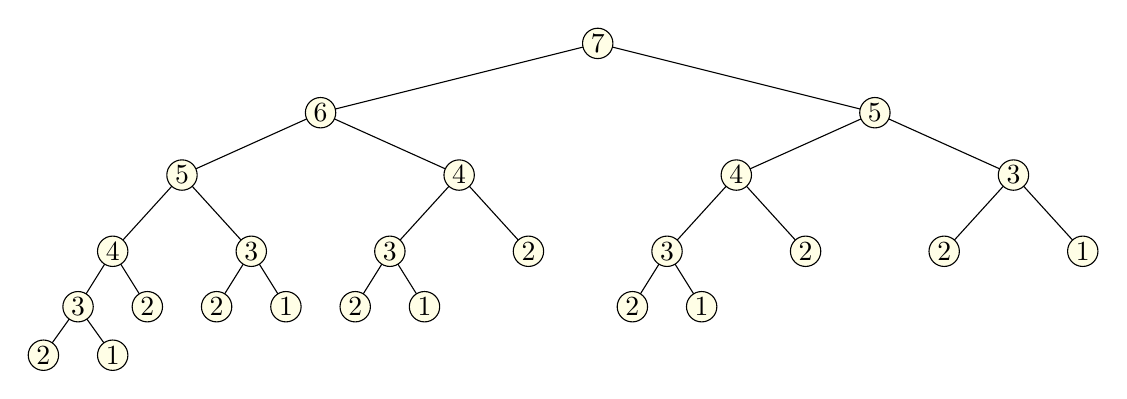
\begin{tikzpicture}[scale=0.88]
  \foreach \y/\lst[count=\j] in {
    0/{0.5,1.5},
    0.7/{1,2,3,4,5,6,9,10},
    1.5/{1.5,3.5,5.5,7.5,9.5,11.5,13.5,15.5},
    2.6/{2.5,6.5,10.5,14.5},
    3.5/{4.5,12.5},
    4.5/{8.5}
  }{
    \foreach \x[count=\i] in \lst {
       \coordinate (p\j\i) at (\x,\y);
       %\pgfmathtruncatemacro{\tmp}{20*\j}
       %\filldraw[fill=black!\tmp] (p\j\i) circle (0.1);
    }
  }
  \foreach \i/\j/\k in {2/1/1,2/1/2,3/1/1,3/1/2,3/2/3,3/2/4,3/3/5,3/3/6,3/5/7,3/5/8,
  4/1/1,4/1/2,4/2/3,4/2/4,4/3/5,4/3/6,4/4/7,4/4/8,5/1/1,5/1/2,5/2/3,5/2/4,6/1/1,6/1/2}{
    \pgfmathtruncatemacro{\tmp}{\i-1}
    \draw (p\i\j)--(p\tmp\k);
  }
  \foreach \lst[count=\i] in {{2,1},{3,2,2,1,2,1,2,1},{4,3,3,2,3,2,2,1},{5,4,4,3},{6,5},{7}} {
    \foreach \v[count=\j] in \lst {
      \node[circle,draw=black,fill=yellow!10, inner sep=1pt] at (p\i\j) {\vb{\v}};
    }
  }
\end{tikzpicture}}


Keď máme dva programy, ako môžeme povedať, ktorý z nich je rýchlejší?
Keby som ti povedal, že vyrátať 37. Fibonacciho číslo mi tvalo 140 ms, nič ti to nepovie,
lebo to závisí od toho, aký mám rýchly počítač. Hlavný problém s funkciou \vb{Fib2} nebol 
v konkrétnych časoch, ale v tom, že sa príliš rýchlo zväčšovali. Chceme teda vymyslieť 
spôsob, ako povedať, ako rýchlo rastie čas programu v závislosti od veľkosti vstupu.
Ukážeme si to na príklade. Povedzme, že už máme načítané pole \vb{a},
v ktorom je $n$ čísel, každé
z nich z rozsahu $0,\ldots,999$. 
Chcem ho preusporiadať tak, aby bolo v poradí od najväčšieho čísla po najmenšie.
Podobný problém si už riešil v úlohách~\ref{uloha:sort1} a \ref{uloha:sort2}, 
teraz skúsme trochu iný prístup, vlastne dva.


\indexItem{Alg}{Insertion Sort}
Prvý program je tzv. {\em Insertion Sort}. Idea je takáto: budeme sa snažiť
prehadzovať prvky v poli tak, aby nakoniec polo utriedené. Algoritmus bude pracovať v
kolách. Na začiatku $i$-teho kola chceme, aby platilo, že prvých $i$ pozícií je
utriedených. Na začiatku prvého kola to platí -- prvý jeden prvok je utriedený vždy.
Ak sa nám podarí, aby to platilo aj po $n$ kolách, budeme mať utriedených
prvých $n$ pozícií, t.j. celé pole. Predpokladajme teraz, že sme na začiatku $i$-teho kola.
Skontrolujeme, či je prvok \vb{a[i]} je menší, ako \vb{a[i-1]}. 
Ak áno, môžeme toto kolo skončiť,
lebo prvých $i+1$ prvkov je utriedených. Ak nie, vymeníme prvky \vb{a[i]} a 
\vb{a[i-1]}
a skontrolujeme, či je \vb{a[i-1]} menší ako \vb{a[i-2]}. Takto pokračujeme ďalej, kým
nedostaneme prvok \vb{a[i]} na správne miesto:


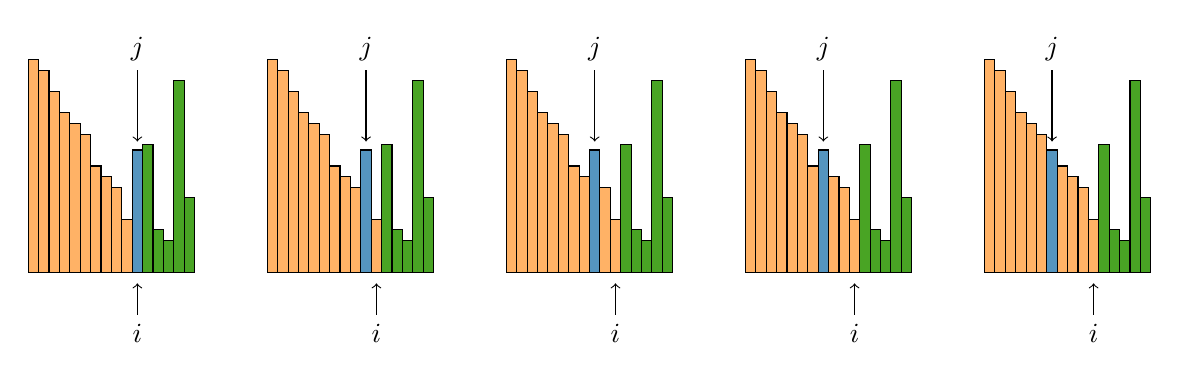
\begin{tikzpicture}[xscale=0.132,yscale=0.135]
  \def\bar(#1,#2)#3{
    \filldraw[draw=black,fill=#3](#1,0) rectangle (#1+1,#2);
  }
  \def\prf{orange!60!white}
  \def\rst{rgb:green,5;yellow,4;blue,2;black,3}
  \def\act{rgb:blue,5;green,3;white,4}
  \def\base{
    \foreach \x[count=\i] in {20,19,17,15,14,13} {
      \bar(\i,\x){\prf}
    }
    \foreach \x[count=\i] in {12,4,3,18,7} {
      \bar(\i+11,\x){\rst}
    }
    \draw [<-, shorten <= 4] (11.5,0) -- (11.5,-4) node [anchor=north]{$i$};
  }
  \def\dj#1{  
  \draw [<-, shorten <= 5] (#1+.5,11) -- (#1+.5,19) node [anchor=south]{$j$};
  }
  \def\sh{23}

  \begin{scope}[shift={(0,0)}]
    \base
    \foreach \x[count=\i] in {10,9,8,5} {
      \bar(\i+6,\x){\prf}
    }
    \bar(11,11.5){\act}
    \dj{11}
  \end{scope}

  \begin{scope}[shift={(\sh,0)}]
    \base
    \foreach \x[count=\i] in {10,9,8} {
      \bar(\i+6,\x){\prf}
    }
    \bar(10,11.5){\act}
    \bar(11,5){\prf}
    \dj{10}
  \end{scope}

  \begin{scope}[shift={(2*\sh,0)}]
    \base
    \foreach \x[count=\i] in {10,9} {
      \bar(\i+6,\x){\prf}
    }
    \bar(9,11.5){\act}
    \bar(10,8){\prf}
    \bar(11,5){\prf}
    \dj{9}
  \end{scope}

  \begin{scope}[shift={(3*\sh,0)}]
    \base
    \bar(7,10){\prf}
    \bar(8,11.5){\act}
    \bar(9,9){\prf}
    \bar(10,8){\prf}
    \bar(11,5){\prf}
    \dj{8}
  \end{scope}

  \begin{scope}[shift={(4*\sh,0)}]
    \base
    \bar(7,11.5){\act}
    \bar(8,10){\prf}
    \bar(9,9){\prf}
    \bar(10,8){\prf}
    \bar(11,5){\prf}
    \dj{7}
  \end{scope}
\end{tikzpicture}


Celá funkcia bude vyzerať takto\footnote{%
  premysli si, čo by sa stalo, keby som vo funkcii \vb{vymen} napísal iba
  \prg!a[i]=a[j]; a[j]=a[i];!
}:


\begin{column}{0.3}
\begin{lstlisting}[] 
void vymen(int i, int j) {
  int x;
  x = a[i];
  a[i] = a[j];
  a[j] = x;
}
\end{lstlisting}
\end{column}
\hfil
\begin{column}{0.55}
\begin{lstlisting}[] 
void InsertSort(int n) {
  int i, j;
  for (i = 1; i < n; i++)
    for (j = i; j > 0 && a[j - 1] < a[j]; j--) 
      vymen(j - 1, j);
}
\end{lstlisting}
\end{column}



\indexItem{Alg}{CountSort}
Druhý program, tzv. {\em CountSort} 
vychádza z toho, že vieme, že vstupné čísla sú z malého rozsahu
(od 0 do 999). Vyrobíme si pomocné pole \prg!pocty[1000]!, v ktorom si budeme
pamätať počty jednotlivých prvkov (\prg!pocty[i]==j! znamená, že sa v poli vyskytuje
\vb{j}-krát hodnota \vb{i}). Takže raz prejdeme vstupným poľom a zistíme počty
a potom len zapíšeme správny počet hodnôt takto:\\


\vbox{
\begin{lstlisting}[] 
void CountSort(int n) {
  int pocty[1000];
  int i, c;

  for (i = 0; i < 1000; i++) pocty[i] = 0;
  for (i = 0; i < n; i++) pocty[a[i]]++;
  i = 0;
  for (c = 999; c>=0 ; c--)
    while (pocty[c] > 0) {
      a[i] = c;
      i++;
      pocty[c]--;
    }
}
\end{lstlisting}
}


Teraz som spravil to, že som oba programy veľakrát spustil na rôznych poliach
a meral im čas. Výsledky sú v nasledovných grafoch\footnote{Vyzerajú síce podobne, 
ale všimni si, že obrázok vľavo je v sekundách a vpravo v mikrosekundách.}

\if\longCharts1

\begin{tikzpicture}[scale=0.9]
\begin{axis}[
  title={InsertSort},
  width=0.5*\textwidth, 
  height=10cm,
  xlabel=$n$,
  ylabel=čas (s),
  scaled x ticks=false,
  scaled y ticks=false,
  domain=0:20000,
  xmin=0,
  xmax=20000,
  /pgf/number format/.cd,
        1000 sep={}
]
  \addplot+[only marks, mark size=0.4pt, mark options={
    draw=orange!80!white,
    fill=red!80!orange
  }
  ] 
  table [y expr=\thisrow{t}/1000000, x=n, ]{data/is.dat};
  \addplot[no markers,red!50!white]{0.0000000027*x*x+0.01};
\end{axis}
\end{tikzpicture}
\hfill
\begin{tikzpicture}[scale=0.9]
\begin{axis}[
  title={CountSort},
  width=0.5*\textwidth, 
  height=10cm,
  xlabel=$n$,
  ylabel=čas ($\mu$s),
  scaled x ticks=false,
  scaled y ticks=false,
  domain=0:20000,
  xmin=0,
  xmax=20000,
  /pgf/number format/.cd,
        1000 sep={}
]
  \addplot+[only marks, mark size=0.4pt, mark options={
    draw=cyan!80!white,
    fill=blue!80!cyan
  }
  ] 
  table [y=t, x=n ]{data/cs.dat};
  \addplot[no markers,blue!50!white]{0.015*x+25};
\end{axis}
\end{tikzpicture}
\fi

\indexItem{Alg}{lineárna, kvadratická a exponenciálna zložitosť}
Z grafov vidno, že obom programom väčšie vstupy trvajú dlhšie, ale aj na rovnako dlhých
vstupoch môžu bežať rôzne dlho (podľa toho, aké konkrétne čísla v tom poli sú).
Ničmenej všetky body na ľavom obrázku sa dajú schovať pod parabolu\footnote{%
  \indexItem{Mat}{parabola}
  graf funkcie $y=ax^2+b$ pre nejaké čísla $a$, $b$} a všetky body vpravo 
  pod priamku. Preto hovoríme, že InsertSort má {\em kvadratickú zložitosť}, kým
CountSort má {\em lineárnu}.


Je lineárny program \footnote{Mal by som písať poriadne ``program s lineárnou časovou zložitosťou''. Označenie ``lineárny program'' znamená v matematike čosi úplne iné, ale teraz nám to nevadí.} 
vždy lepší ako kvadratický?
Predpokladajme, že máme lineárny program
${\mathcal A}$, ktorého čas na vstupe veľkosti
$n$ je najviac $42n+200$. Majme hocijaký kvadratický program ${\mathcal B}$,
ktorého čas na vstupe veľkosti $n$ je $an^2+b$ pre nejaké čísla $a$, $b$. 
Pre malé hodnoty $n$ môže byť program ${\mathcal B}$ rýchlejší. Ale existuje
$n$, kedy $24n+200=an^2+b$, a od tohto $n$ ďalej už bude rýchlejší program
${\mathcal A}$. 


\centerline{
  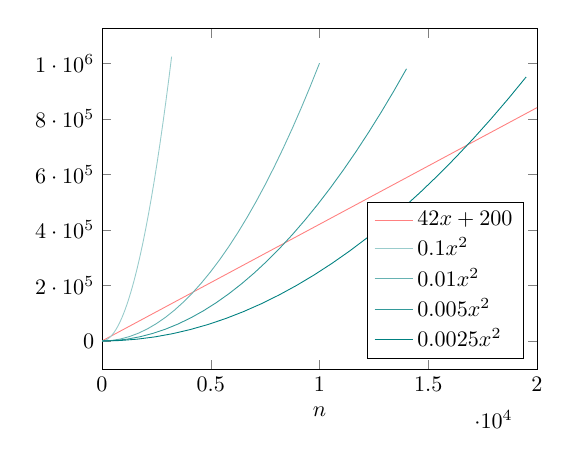
\begin{tikzpicture}[scale=0.8]
\begin{axis}[
  width=0.7*\textwidth, 
  height=7cm,
  xlabel=$n$,
  %scaled x ticks=false,
  scaled y ticks=false,
  domain=0:20000,
  xmin=0,
  xmax=20000,
  /pgf/number format/.cd,
        1000 sep={},
  legend cell align={left},
  legend pos = south east
]
  \addplot[no markers,red!50!white]{42*x+200};
  \addlegendentry{$42x+200$}
  \addplot[domain=0:3200,no markers,teal!40!white]{0.1*x*x};
  \addlegendentry{$0.1x^2$}
  \addplot[domain=0:10000,no markers,teal!60!white]{0.01*x*x};
  \addlegendentry{$0.01x^2$}
  \addplot[domain=0:14000,no markers,teal!80!white]{0.005*x*x};
  \addlegendentry{$0.005x^2$}
  \addplot[domain=0:19500,no markers,teal]{0.0025*x*x};
  \addlegendentry{$0.0025x^2$}
\end{axis}
\end{tikzpicture}}


Inými slovami, pre každý kvadratický program platí, že pre dosť veľké vstupy je
${\mathcal A}$ rýchlejší. Podobne vieme hovoriť o kubických programoch, programoch štvrtého 
stupňa atď. A ako by dopadol program \vb{Fib2}? Jeho zložitosť je až $2^n$: rastie
rýchlejšie, ako akýkoľvek polynóm $x^c$. Takýmto programom hovoríme {\em exponenciálne}.

 
Typický príklad programu s lineárnou zložitosťou je jeden cyklus, ktorý
raz prejde cez vstupné hodnoty a niečo na nich ráta (napr. hľadá maximum): keď bude
vstup dvojnásobne dlhý, program pobeží dvakrát dlhšie -- to je lineárna závislosť.
Dva vnorené cykly takto:\\


\vbox{
\begin{lstlisting}[] 
for (i = 0; i < n; i++)
  for (j = 0; j < n; j++)
    if (i != j) {
      x = a[j] - a[i];
      if (x < 0) x = -x;
      if (x < m) m = x;
    }
\end{lstlisting}
}

sú zas typický príklad kvadratického programu: keď má vstup dĺžku $n$, vnútro cyklu
sa vykoná $n^2$-krát (mimochodom: skús sa zamyslieť, čo ten program robí).
Vnútro cyklu trvá vždy rovnako dlho (je tam len niekoľko priradení a testov), nech je to $s$ milisekúnd.
Čas celého programu preto bude $n^2\cdot s$ milisekúnd, čo je kvadratická závislosť.
Treba byť ale opatrný, nie všetky vnorené cykly znamenajú kvadratickú
zložitosť. Pozrime sa na takýto príklad: v poli \vb{a} je uložených \vb{n}
rôznych čísel. Naším cieľom je nájsť najdlhší úsek, v ktorom sú čísla utriedené od 
najmenšieho. Napr. v poli
{\robotomono 12 \textcolor{teal}{4 5 8} 6 \textcolor{orange}{5 10}
\textcolor{rgb:green,5;yellow,4;blue,2;black,3}{ 9 11 13 14} 3
}
sú tri také úseky označené farebne a najdlhší z nich má dĺžku $4$.


Priamočiary spôsob riešenia je pre každú pozíciu v poli vyskúšať, aký dlhý rastúci úsek 
sa z nej začína. Budeme mať teda jednu premennú \vb{i}, ktorou prejdeme v cykle
cez celé pole a zakaždým v druhom cykle premennou \vb{j} zistíme dĺžku rastúceho úseku.
Napríklad pre $\vb{i}=1$, bude najprv $\vb{j}=2$ a pretože $\vb{a[2]}=5 > 4=\vb{a[1]}$,
\vb{j} sa nastaví na $3$ a cyklus sa zopakuje. Rovnako  $\vb{a[3]}=8 > 5=\vb{a[2]}$,
preto sa cyklus opäť zopakuje a \vb{j} bude $4$. Teraz  $\vb{a[4]}=6 < 8=\vb{a[3]}$,
preto cyklus skončí s hodnotou $\vb{j}=4$. Dĺžka rastúceho úseku so začiatkom
v \vb{i} je preto \vb{j - i}.


\begin{column}{0.45}
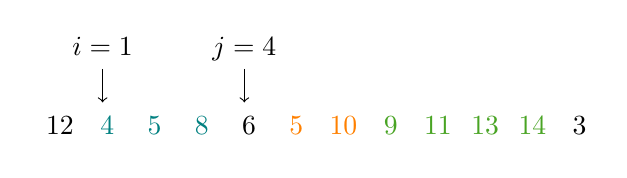
\begin{tikzpicture}[scale=0.6]
  \def\cc{rgb:green,5;yellow,4;blue,2;black,3}
  \foreach \x/\c[count=\i] in {12/black, 4/teal, 5/teal, 8/teal, 6/black, 5/orange, 10/orange, 9/0, 11/0, 13/0, 14/0, 3/black} {
  \draw[draw=none] (\i,0) rectangle node[anchor=center]{\vb{
    \textcolor{\if\c0\cc\else\c\fi}{\x }}} (\i+1,1);
  }
  \draw[->, shorten <= 5] (2.5,2) node[anchor=base]{$\vb{i}=1$}-- (2.5,1);
  \draw[->, shorten <= 5] (5.5,2) node[anchor=base]{$\vb{j}=4$}-- (5.5,1);
\end{tikzpicture}


Program by vyzeral napr. takto:
\end{column}\hfill\begin{column}{0.45}
\begin{lstlisting}[] 
int usek1() {
  int i = 0, j, m = 0;
  while (i < n - 1) {
    j = i + 1;
    while (j < n && a[j] > a[j - 1]) 
      j++;
    if (j - i > m) m = j - i;
    i++;
  }
  return m;
}
\end{lstlisting}
\end{column}

V programe máme dva vnorené cykly. Koľkokrát sa vykoná inštrukcia \vb{j++}
vo vnútornom cykle? Predpokladajme, že na vstupe sú čísla usporiadané vzostupne
\vb{1 2 3 ... $n$}. Na začiatku je \vb{i}=0, takže vnútorný cyklus začína od 0,
a keďže je celé pole rastúce, zopakuje sa $n-1$ krát. Potom sa nastaví
\vb{i}=1 a vnútorný cyklus sa zopakuje $n-2$ krát atď. Celkovo
sa teda vnútorný cyklus zopakuje \indexItem{Mat}{súčet prvých $n$ prirodzených čísel}$(n-1)+(n-2)+(n-3)+\cdots+3+2+1$ krát.
Ako takýto súčet môžeme vyrátať? Stačí si preusporiadať čísla: prvé s posledným
dá dokopy $(n-1)+1=n$. Druhé s predposledným dá $(n-2)+2=n$ atď. Dokopy takto získame
$(n-1)/2$ dvojíc po $n$, teda výsledok\footnote{%
  Toto, čo sme povedali, platí pre nepárne $n$, aby $(n-1)/2$ bolo celé číslo. Ako je to pre
  párne $n$? Dostaneme $(n-2)/2$ dvojíc po $n$ a ešte v strede ostane jedno číslo $n/2$.
  Dokopy to teda bude $n(n-2)/2+n/2=(n^2-2n)/2+n/2=(n^2-2n+n)/2=(n^2-n)/2=n(n-1)/2$,
  takže výsledok sedí aj v tomto prípade.
}je $n(n-1)/2$, čo je kvadratická funkcia.


\begin{column}{0.4}
Vedel by si zložitosť tohoto programu vylepšiť? Stačí si uvedomiť, že veľa roboty 
sa robí zbytočne. Napríklad pre $\vb{i}=1$ skončí vnútorný cyklus s hodnotou
$\vb{j}=4$. Čo sa stane pre $\vb{i}=2$? Vnútorný cyklus opäť príde po $\vb{j}=4$
a potom zastane, lebo nájde menšie číslo  $\vb{a[4]}=6 < 8=\vb{a[3]}$. Samozrejme,
rastúci úsek od $\vb{i}=2$ je kratší. Nás ale zaujíma najdlhší rastúci úsek, preto
nepotrebujeme skúšať $\vb{i}=2$ ani $\vb{i}=3$, ale
najbližšie \vb{i}, ktoré potrebujeme skúsiť je \vb{i = j}. Upravme program takto:
\end{column}\hfill\begin{column}{0.5}
%\vbox{
\begin{lstlisting}[] 
int usek2() {
  int i = 0, j, m = 0;
  while (i < n - 1) {
    j = i + 1;
    while (j < n && a[j] > a[j - 1]) j++;
    if (j - i > m) m = j - i;
    i = j;
  }
  return m;
}
\end{lstlisting}
%}
\end{column}

\vskip 2ex
Zdanlivo je to malá zmena, stále máme dva vnorené cykly, ale vidno, že každá premenná
v poli \vb{a} sa testuje na \vb{a[j] > a[j - 1]} iba raz za celý program (keď sa raz
v nejakom cykle otestuje, ďalšia iterácia vonkajšieho cyklu ju už preskočí). Funkcia
\vb{usek2} má teda lineárnu zložitosť. Naozaj sa ten rozdiel prejaví? 
Skúšal som si merať časy na rôznych vstupoch. Pre funkciu \vb{usek1} je najhoršie,
ak je vstup celý rastúco utriedený, lebo vtedy vnútorný cyklus vždy prejde až do konca.
Tento prípad bol tak pomalý, že všetky ostatné som musel stokrát spomaliť, aby na
obrázku bolo vôbec niečo vidno. Okrem toho som skúšal aj náhodné postupnosti pre rôzne dĺžky
(pre každú dĺžku som zobral priemer 100 náhodných vstupov). Výsledky vyzerajú takto:

\vskip 2ex
\centerline{
\begin{tikzpicture}
\begin{axis}[
  %title={CountSort},
  width=\textwidth, 
  height=10cm,
  xlabel=$n$,
  ylabel=čas (ms),
  scaled x ticks=false,
  scaled y ticks=false,
  y tick label style={
        /pgf/number format/.cd,
            fixed,
            fixed zerofill,
            precision=1,
        /tikz/.cd
    },
  legend cell align={left},
  legend pos = north west,
  %scale only axis,
  %separate axis lines,
  %domain=0:50000,
  %xmin=0,
  %xmax=50000,
  ymin=0,
  %ymax=20,
  /pgf/number format/.cd,
        1000 sep={}
]
  \addplot+[no markers,orange!80!white] table 
  [y expr=\thisrow{max1}/1000000, x=n ]{data/usek.dat};
  \addlegendentry{funkcia \vb{usek1}, utriedený vstup}
  \addplot+[no markers,orange!20!white] table 
  [y expr=\thisrow{avg1}/10000, x=n ]{data/usek.dat};
  \addlegendentry{funkcia \vb{usek1}, náhodný vstup, stokrát spomalená}
  \addplot+[no markers,blue!80!cyan] table 
  [y expr=\thisrow{max2}/10000, x=n ]{data/usek.dat};
  \addlegendentry{funkcia \vb{usek2}, utriedený vstup, stokrát spomalená}
  \addplot+[no markers,blue!20!cyan] table 
  [y expr=\thisrow{avg2}/10000, x=n ]{data/usek.dat};
  \addlegendentry{funkcia \vb{usek2}, náhodný vstup, stokrát spomalená}
\end{axis}
\end{tikzpicture}
}


Na to, aby sme určili zložitosť (t.j. aby sme vedeli povedať, či sa čas behu programu
v závislosti od veľkosti vstupu vždy
zmestí pod priamku, parabolu, atď) treba vedieť, čo je pre program najhorší vstup
a celé to môže byť aj celkom ťažké. Ale je treba si zapamätať, že tá istá úloha sa dá naprogramovať rôznymi spôsobmi 
a veľmi záleží na tom, ako to urobíš. Pri súťažiach je pre úlohy väčšinou stanovený aj 
časový limit: ak tvoj program neskončí dosť rýchlo, testovač ho preruší a neuzná 
(dostaneš odpoveď TLE = {\em time limit exceeded}).
V tom prípade máš dve možnosti: skúsiť nejaké finty, ako veci trochu zrýchliť, alebo
sa zamyslieť nad úplne iným spôsobom, ako úlohu naprogramovať.


Tu je zopár úloh, ktoré sa dajú naprogramovať rôzne rýchlo. Skús nájsť najrýchlejší spôsob.

\begin{uloha}
  Na vstupe je číslo $n$, potom pole $n$ čísel a potom $n$ otázok, pričom každá otázka
  pozostáva z dvoch čísel \vb{i}, \vb{j}, pričom platí $0\le i\le j<n$. 
  Úlohou je napísať program, ktorý pre každú
  otázku $i,j$ vypíše súčet $\vb{a}[\vb{i}]+\vb{a}[\vb{i}+1]+\cdots+\vb{a}[\vb{j}]$.
  Napr. pre pole \vb{5 7 -1 8 3 -2} a otázku \vb{1 3} je odpoveď
  $7-1+8=14$.
\end{uloha}

\begin{uloha}
  Na vstupe je číslo $n$, utriedené pole $n$ čísel a číslo $k$. Úlohou je napísať
  program, ktorý nájde počet dvojíc čísel, ktorých rozdiel je $k$.
  Napr. pre pole \vb{3 4 7 7 8 11 12 16} a $k=5$ je odpoveď $3$, lebo v poli
  sú dvojice $(3,8)$, $(7,12)$, $(11,16)$.
\end{uloha}


Na záver ešte jedna ukážka, ktorú použijeme aj v ďalšej kapitole.

\begin{uloha}
 $n$ klaunov s výškami $1,2,\ldots,n$ sa postavilo do radu v nejakom poradí. 
  Každý z nich hodil smerom doprava šľahačkovú tortu, ktorá dopadla na 
  najbližšieho vyššieho klauna (ak tam taký nebol, torta
  preletela preč). Napíš program, ktorý načíta číslo $n$
  a poradie klaunov a vypíše, koľko najviac zásahov nejaký klaun dostal.
  Napr. pre $\vb{n}=5$ a poradie \vb{3 2 5 4 1} je odpoveď $2$, lebo na klaunovi
  $5$ pristane torta od dvojky aj trojky.
\end{uloha}

Priamočiary spôsob riešenia je napísať si funkciu, ktorá pre dvojicu klaunov 
\vb{j} a \vb{i} povie, či klaun \vb{j} trafí klauna \vb{i}. To je jednoduché:
stačí zistiť, či je medzi nimi niekto vyšší:

\begin{column}{0.5}
\begin{lstlisting}[] 
bool trafi(int j, int i) {
  int k;
  if (a[i] < a[j]) return false;
  for (k = j + 1; k < i; k++)
    if (a[k] > a[j]) return false;
  return true;
}
\end{lstlisting}
\end{column}\hfill\begin{column}{0.5}
\centerline{
  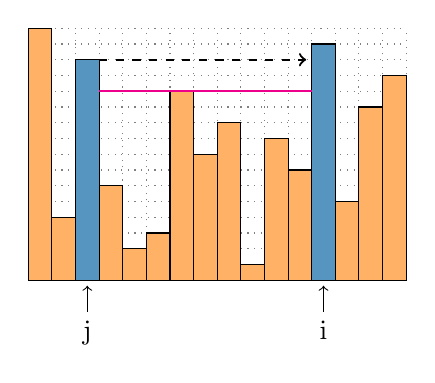
\begin{tikzpicture}[xscale=0.3,yscale=0.2]
  \draw[dotted,gray,thin] (1,0) grid (17,16);
  \def\bar(#1,#2)#3{
    \filldraw[draw=black,fill=#3](#1,0) rectangle (#1+1,#2);
  }
  \def\prf{orange!60!white}
  \def\rst{rgb:green,5;yellow,4;blue,2;black,3}
  \def\act{rgb:blue,5;green,3;white,4}
    \foreach \h [count=\i] in {16,4,14,6,2,3,12,8,10,1,9,7,15,5,11,13} {
    \bar(\i,\h){\prf}
  }
  \bar(13,15){\act}
  \draw[->,shorten >= 2](13.5,-2) node[anchor=north]{\vb{i}} -- (13.5,0);
  \bar(3,14){\act}
  \draw[->,shorten >= 2](3.5,-2) node[anchor=north]{\vb{j}} -- (3.5,0);

    \draw[magenta,thick](4,12) -- (13,12);

    \draw[->,thick,shorten >=2, dashed](4,14)--(13,14);  
  \end{tikzpicture}
}
\end{column}




S pomocou tejto funkcie už ľahko otestujeme všetky dvojice klaunov:

\phantom{aaa}


\vbox{
\begin{lstlisting}[] 
int klauni1() {
  int i, j, max = 0;
  for (i = 1; i < n; i++) {  // skúšame každého klauna
    int hits = 0;            // koľko zásahov dostal
    for (j = 0; j < i; j++)  // všetci klauni naľavo od i
      if (trafi(j, i)) hits++;
    if (hits > max) max = hits;
  }
  return max;
}
\end{lstlisting}
}

\phantom{aaa}

Akú má tento program zložitosť? Funkcia \vb{trafi(j,i)} urobí $i-j$
operácií. Na otestovanie klauna $i$ voláme \vb{trafi(j,i)} pre všetky
menšie \vb{j}, preto ten test spotrebuje $i+(i-1)+(i-2)+\cdots+1$ operácií.
Takýto súčet si už rátal, je to $(i+1)i/2$. Napokon toto celé robíme pre 
všetkých klaunov, teda dokopy máme \hbox{$(1+1)1/2+(2+1)2/2+(3+1)3/2+\cdots+n(n-1)/2$}
operácií. Presne zrátať tento súčet je trochu ťažšie\footnote{výsledok
je $\frac{1}{6}n(n+1)(n+2)$}, ale ľahko môžeš odhadnúť, že $(i+1)i/2>i^2/2$,
a preto v súčte je aspoň $(n-1)/2$ členov, z ktorých každý je väčší
ako $(n/2)^2/2$. Dokopy je teda zložitosť väčšia ako
$\frac{n-1}{2}\frac{(n/2)^2}{2}=\frac{1}{4}(n-1)n^2/4>\frac{1}{16}n^3$.
Takáto zložitosť sa volá {\em kubická} (čas sa vždy zmestí pod graf funkcie
$an^3+b$ pre nejaké čísla $a,b$). Vzťah medzi kubickou a kvadratickou zložitosťou
je rovnaký ako medzi kvadratickou a lineárnou: hocijaký kvadratický program 
začne byť pre dosť veľké vstupy lepší ako daný kubický.

 Poďme to trochu vylepšiť. Kde sa robí zbytočná robota? Vo funkcii \vb{trafi}
zakaždým hľadáme najvyššieho klauna medzi \vb{i} a \vb{j}. Túto prácu si vieme ušetriť,
ak si ho budeme pamätať priebežne a iba aktualizovať. Vo vylepšenej verzii budeme
opäť prechádzať v cykle cez všetkých klaunov (na to bude
premenná \vb{i}) a pre každého zistíme, koľko zásahov dostane. 
To budeme robiť v druhom cykle (s premennou \vb{j}).
Budeme postupne prechádzať klaunov od $i-1$ smerom doľava,
až kým neprídeme na začiatok, alebo nestretneme väčšsieho klauna (spoza neho
už klauna \vb{i} nikto netrafí). Každý klaun \vb{j}, ktorého takto stretneme,
trafí klauna \vb{i}, ak je vyšší, ako najvyšší klaun, ktorý je medzi nimi. Jeho výšku
si budeme pamätať v premennej \vb{v} a vždy, keď stretneme klauna
\vb{j}, ktorý je vyšší ako \vb{v}, si ju upravíme.

\phantom{aaa}


\centerline{
  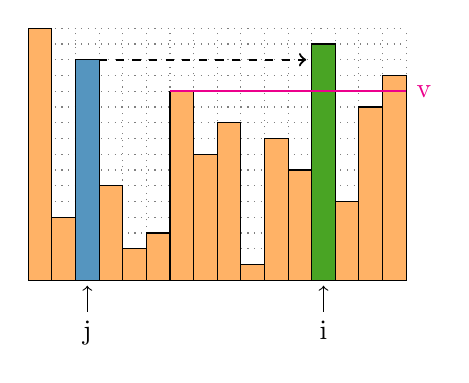
\begin{tikzpicture}[xscale=0.3,yscale=0.2]
  \draw[dotted,gray,thin] (1,0) grid (17,16);
  \def\bar(#1,#2)#3{
    \filldraw[draw=black,fill=#3](#1,0) rectangle (#1+1,#2);
  }
  \def\prf{orange!60!white}
  \def\rst{rgb:green,5;yellow,4;blue,2;black,3}
  \def\act{rgb:blue,5;green,3;white,4}
    \foreach \h [count=\i] in {16,4,14,6,2,3,12,8,10,1,9,7,15,5,11,13} {
    \bar(\i,\h){\prf}
  }
  \bar(13,15){\rst}
  \draw[->,shorten >= 2](13.5,-2) node[anchor=north]{\vb{i}} -- (13.5,0);
  \bar(3,14){\act}
  \draw[->,shorten >= 2](3.5,-2) node[anchor=north]{\vb{j}} -- (3.5,0);

    \draw[magenta,thick](7,12) -- (17,12) node[anchor=west]{\vb{v}};

    \draw[->,thick,shorten >=2, dashed](4,14)--(13,14);  
  \end{tikzpicture}
}

\phantom{aaa}


\vbox{
\begin{lstlisting}[] 
int klauni2() {
  int i, j, max = 0;
  for (i = 1; i < n; i++) {  // skúšame každého klauna
    int hits = 0,            // koľko zásahov dostal
        v = 0;               // najvyšší klaun medzi nimi
    for (j = i - 1; j >= 0 && a[j] < a[i]; j--)  // skúšame vľavo
      if (a[j] > v) {                            // trafí ?
        hits++;                                  // zarátame zásah
        v = a[j];                                // upravíme výšku
      }
    if (hits > max) max = hits;  // pamätáme si najzapatlanejšieho
  }
  return max;
}
\end{lstlisting}
}

\phantom{aaa}


Akú má ztento program ložitosť? Podobne, ako v predchádzajúcom príklade, najhorší prípad je, 
keď sú klauni utriedení: vtedy vnútorný cyklus pôjde zakaždým až po začiatok,
a teda celkový počet opakovaní bude \hbox{$1+2+3+\cdots+(n-2)+(n-1)$,} čo je kvadraticky
veľa.
